% main.tex — arXiv-Papier für „Rechnen auf einem chaotischen Substrat"
% Bauen:  pdflatex main && pdflatex main   (Literatur inline via thebibliography, kein bibtex)
%         (oder: latexmk -pdf main)
% Abbildungen: python3 make_figures.py .  (erzeugt fig_bistabilitaet.pdf, fig_lyapunov.pdf)
%
% arXiv-Hinweise (beim Einreichen):
%   - Primäre Kategorie cs.ET (Emerging Technologies), sekundär nlin.CD (Chaotic Dynamics).
%   - Lizenz: Paper unter arXiv-Standardlizenz; der Code bleibt CC BY-NC 4.0 (separat im Repo).
%   - Abbildungen als PDF (nicht PNG) einbetten; die Quell-PNGs liegen im Repo unter files (1)/.
\documentclass[11pt]{article}

\usepackage[T1]{fontenc}
\usepackage[utf8]{inputenc}
\usepackage{amsmath,amssymb}
\usepackage{graphicx}
\usepackage{booktabs}
\usepackage[hidelinks]{hyperref}

\title{Universal Computation on a Chaotic Substrate:\\ a Feasibility Proof with a Measured Contracting Operating Point}

\author{Jakob Notter\thanks{Independent researcher, \href{https://github.com/jnrabit}{github.com/jnrabit}}}

\date{\today}

\begin{document}
\maketitle

\begin{abstract}
We show that a field of coupled Lorenz systems, driven by a small sinusoidal term, can serve
as a complete computing substrate. Each cell consists of two coupled Lorenz halves whose
driven $w$-component develops two stable poles near $\pm 363$, forming a bistable switch that
stores bits. A single regenerative gate term, which pulls a cell's $w$-component toward the
anchor $\operatorname{sign}(\mathrm{NET})\cdot 363$, realizes functionally complete logic;
because every output is re-regenerated onto the anchor, gates compose into arbitrary
combinational networks with no accumulation of error over depth. We verify storage,
AND/OR/NAND/XOR/XNOR logic, multi-stage chains, and a non-trivial application---a
self-consistent knowledge store that admits fact triples and rejects contradictions---each
against an independent reference. The stability underlying all correctness properties is not
assumed but measured: Benettin's method yields a largest Lyapunov exponent
$\lambda = -0.69$ at the operating point ($-1.23$ with the gate term), versus $+0.91$ for the
undriven system, so the operating point contracts and actively extinguishes perturbations.
Coupling the substrate to real hardware entropy (GPU temperature, CPU-cycle jitter) keeps the
logic intact while making runs genuinely non-deterministic. This is a feasibility proof:
computation on this substrate is possible in principle and in full, while any practical
advantage would require physical analog hardware at scale, outside the scope of this work.
\end{abstract}

\section{Introduction}
Computation on physical substrates that are not silicon logic has a long history. Two strands are
closest to the present work. \emph{Reservoir computing} \cite{jaeger2001,maass2002} exploits the
transient dynamics of a fixed, often chaotic recurrent network: only a linear readout is trained,
and the substrate itself is treated as an untrained black box. \emph{Chaos computing}
\cite{munakata2002,ditto2008} instead encodes logic directly in the state of a chaotic element,
using the attractor's basins as the bit and steering it via parameters. Both leave a question open:
is the computation an emergent, robust property of the substrate itself, or an artefact of the
readout and control layered on top of it?

This work answers that question for one concrete substrate by carrying the argument through end to
end. We take a field of coupled Lorenz systems \cite{lorenz1963}, add a small periodic drive, and
find that the operating point becomes \emph{contracting}---its largest Lyapunov exponent is
\emph{measured} to be negative ($\lambda\approx-0.69$), in contrast to $+0.91$ for the undriven
system. From this single measured fact all correctness properties follow as consequences: a
bistable one-bit memory, functionally complete logic realized by one regenerative gate rule, gates
that compose into arbitrary combinational networks with no error accumulation over depth, Turing
capability, parallel scaling to thousands of cells, and coupling to genuine hardware entropy without
loss of logic.

The contributions are (i) a complete, every-stage-verified feasibility proof that a chaotic
substrate can compute universally, and (ii) the demonstration that its correctness rests on a single
physically measurable property---a contracting operating point---rather than on the choice of readout
or control. We are explicit about what is \emph{not} shown: simulated on conventional hardware the
substrate is slower than direct logic, and the potential advantages (entropy-in-computation,
intrinsic error correction, in-memory computation) would materialize only in physical analog hardware
at scale.

\section{The substrate}
A cell consists of two coupled Lorenz half-systems (eight state variables
$x_1,y_1,z_1,w_1,x_2,y_2,z_2,w_2$). Per half-system:
\begin{align}
  \dot{x} &= \sigma(y-x), \nonumber\\
  \dot{y} &= x(\rho-z) - y + W\,w, \nonumber\\
  \dot{z} &= xy - \beta z, \nonumber\\
  \dot{w} &= -w + xz - W\,y,
\end{align}
with $\sigma=10$, $\rho=28$, $\beta=8/3$ (the classical chaotic Lorenz regime), integrated with
RK4 and $dt=0.005$. Cells couple through a mean field on the $x$-channels
($\dot{x}_1 \mathrel{+}= K(\bar{x}_1 - x_1)$, $K=0.05$), where $\bar{x}$ is a \emph{snapshot} of
all cells at tick start, making the coupling order-independent and exactly parallelizable.

The term $W$ is the drive,
$W = 0.225 + 0.018\sin(1.8\,t) + \dots$. At this operating point the $w$-component develops
\emph{two stable poles near $\pm 363$} --- an emergent bistable switch, not hard-coded.

\section{Bit and memory}
The two $\pm 363$ poles serve as the bit. A short state perturbation sets the bit (flips the cell
into the desired wing), where it is then held by itself --- a non-volatile one-bit memory from
pure dynamics (Fig.~\ref{fig:bistability}).
\begin{figure}[t]
  \centering
  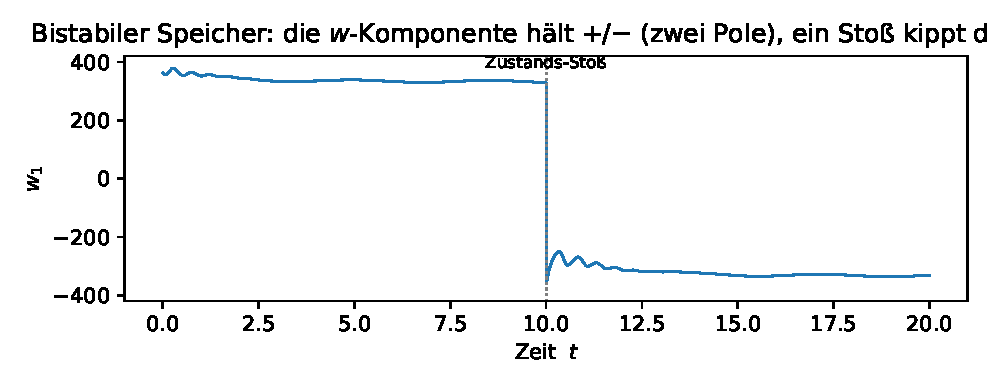
\includegraphics[width=\linewidth]{fig_bistabilitaet.pdf}
  \caption{Bistable memory. The $w_1$-component of one cell settles onto one of two stable poles
  and holds it; a state impulse (dotted line) flips the bit into the opposite pole, where it is
  again held. The bit is a stable fixed point of the driven dynamics, not an encoded constant.}
  \label{fig:bistability}
\end{figure}

\section{Functionally complete logic}
A gate is a feedback term pulling a cell's $w$-component toward a regenerated target:
\begin{equation}
  \dot{w}_1 \mathrel{+}= g_K\big(\operatorname{sign}(\mathrm{NET})\cdot 363 - w_1\big),
\end{equation}
where $\mathrm{NET}$ is the weighted sum of gate inputs plus bias. This single term realizes
AND, OR, NAND, etc.; a READ gate copies a bit non-destructively.

\textbf{The regeneration rule.} Regenerating the output onto the fixed anchor
$\operatorname{sign}(\mathrm{NET})\cdot 363$ (rather than passing $\mathrm{NET}$ through raw) is
the central construction decision: it makes gates \emph{chainable}, because every output is
again a full-saturated $\pm 363$ bit. This rule reappears at three independent places
(\S\ref{sec:scaling}, \S\ref{sec:contraction}, \S\ref{sec:entropy}).

\section{Chaining and Turing capability}
Multi-stage networks are built by holding intermediate results as cells and reading them as
inputs to the next stage (verified: XNOR/XOR, three stages; a four-stage conflict condition).
\emph{Depth independence (measured):} no error accumulates over depth --- the deepest network
was the cleanest (bit-exact against reference), because each stage re-regenerates onto the
$\pm 363$ fixed point. A pulse-clocked program counter, storing control unit, and conditional
branching were shown on the precursor substrate, together establishing Turing capability. One
architectural limit is stated explicitly: the substrate cannot clock itself; the clock is
external.

\section{Scaling on parallel hardware}
\label{sec:scaling}
The dynamics were ported to an OpenCL GPU data path (double precision) and verified in stages:
dynamics bit-near ($\approx 10^{-13}$ over $10^3$ steps); the gate primitive \emph{bit-exact}
on the GPU (the $\pm 363$ fixed point absorbs rounding differences); thousands of gates in one
kernel launch; multi-stage nets without the sequential staging the 8-core limit had forced.
A GPU-side reduction removes the per-tick host-readback bottleneck, reaching
$70$--$85$k ticks/s ($5.8\times$ at $N=4096$ cells); the settled conflict check drops to
$\sim 7$\,ms. The register/write wall of the 8-core reference (a few cells) is lifted to thousands
of cells and gates computing concurrently.

\section{The physical root: measured contraction}
\label{sec:contraction}
By Benettin's method (two minimally separated trajectories, $\delta_0=10^{-9}$, renormalized
against saturation):
\begin{center}
\begin{tabular}{lcc}
\toprule
State & $\lambda_{\max}$ & Meaning \\
\midrule
At operating point, in wing & $-0.69$ & contracting \\
In wing, with gate term & $-1.23$ & more strongly contracting \\
Pure Lorenz ($W=0$) & $+0.91$ & diverging (classical chaos) \\
\bottomrule
\end{tabular}
\end{center}
The damping timescale $1/|\lambda| \approx 160$--$290$ steps quantitatively explains the
measured settling floor of $\sim 750$ steps. Even a generic start state falls into the
contracting well --- the stability is a \emph{global} property of the operating point. The full
8-dimensional spectrum (Fig.~\ref{fig:lyapunov}) confirms this: at the operating point all eight
exponents are negative, so the Kolmogorov--Sinai entropy $h_{\mathrm{KS}}=\sum_i \lambda_i^+$
\cite{pesin1977} vanishes, whereas the free Lorenz system has two positive exponents and
$h_{\mathrm{KS}}\approx 1.8$. The drive turns a chaotic process into a regular one.
\begin{figure}[t]
  \centering
  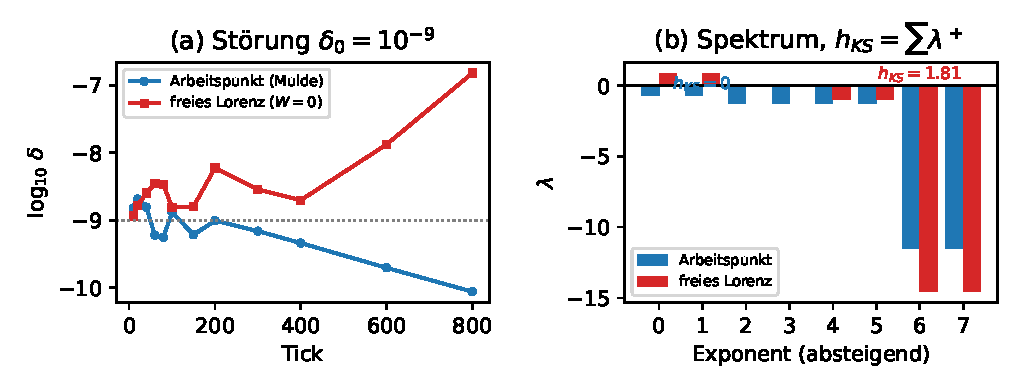
\includegraphics[width=\linewidth]{fig_lyapunov.pdf}
  \caption{Measured contraction. (a) Two nearly identical trajectories ($\delta_0=10^{-9}$) stay
  together at the operating point but separate exponentially in the free Lorenz system. (b) The
  full Lyapunov spectrum: all eight exponents are negative at the operating point
  ($h_{\mathrm{KS}}=0$), whereas the undriven system has two positive exponents
  ($h_{\mathrm{KS}}\approx 1.8$).}
  \label{fig:lyapunov}
\end{figure}

\section{Coupling to real physics}
\label{sec:entropy}
The substrate was coupled to real hardware entropy of the host machine: GPU temperature (slow
drift) and CPU-cycle jitter (fast micro-variance). The logic remains intact (structurally: the
drive deepens the well), while the system becomes non-deterministic --- repeated runs differ
measurably, whereas uncoupled runs are bit-identical. This is the one place where the substrate
does something digital logic does not do by itself: carry physical noise \emph{in} the
computation.

\section{A real application (illustration)}
The core operation of a knowledge store with consistency checking: a new fact triple is checked
against the existing triples for contradiction (same subject+predicate, different object), in
parallel, in one pass; consistent triples are admitted, contradictory ones reported. Extended to
rule operations (retraction, staging/ratification). Verified against an independent reference
up to several hundred triples, with multi-bit-coded entities.

\section{Scope and limits (honest)}
\emph{Proven:} a chaotic Lorenz substrate can compute universally, with the stability measured
as a contracting dynamics, every stage verified against a reference. \emph{Not proven:} a
practical advantage. Three plausible candidates --- (a) entropy-in-computation for
crypto/stochastic methods, (b) intrinsic error correction by the contracting well, (c) compute
and store in the same place --- are all unrealizable \emph{in simulation} and would only appear
in real analog hardware at scale.

\section{Reproducibility}
All measurements were run against an unchanged reference implementation (integrity hash-checked
before and after each measurement). Code and full development log:
\url{https://github.com/jnrabit/chaos-rechenwerk}; DOI:
\href{https://doi.org/10.5281/zenodo.20829024}{10.5281/zenodo.20829024}.

\bibliographystyle{plain}
\begin{thebibliography}{9}
\bibitem{notter2026chaos} J.~Notter,
  \emph{Rechnen auf einem chaotischen Substrat --- ein Machbarkeitsbeweis},
  2026, DOI: \href{https://doi.org/10.5281/zenodo.20829024}{10.5281/zenodo.20829024}.

\bibitem{lorenz1963} E.~N.~Lorenz,
  Deterministic nonperiodic flow,
  \emph{J. Atmos. Sci.} \textbf{20}, 130--141 (1963).

\bibitem{jaeger2001} H.~Jaeger,
  The ``echo state'' approach to analysing and training recurrent neural networks,
  GMD Report 148, German National Research Center for Information Technology (2001).

\bibitem{maass2002} W.~Maass, T.~Natschläger, H.~Markram,
  Real-time computing without stable states: a new framework for neural computation based on
  perturbations, \emph{Neural Comput.} \textbf{14}, 2531--2560 (2002).

\bibitem{munakata2002} T.~Munakata, S.~Sinha, W.~L.~Ditto,
  Chaos computing: implementation of fundamental logical gates by chaotic elements,
  \emph{IEEE Trans. Circuits Syst. I} \textbf{49}, 1629--1633 (2002).

\bibitem{ditto2008} W.~L.~Ditto, K.~Murali, S.~Sinha,
  Chaos computing: ideas and implementations,
  \emph{Phil. Trans. R. Soc. A} \textbf{366}, 653--664 (2008).

\bibitem{benettin1980} G.~Benettin, L.~Galgani, A.~Giorgilli, J.-M.~Strelcyn,
  Lyapunov characteristic exponents for smooth dynamical systems and for Hamiltonian systems,
  \emph{Meccanica} \textbf{15}, 9--20 (1980).

\bibitem{pesin1977} Ya.~B.~Pesin,
  Characteristic Lyapunov exponents and smooth ergodic theory,
  \emph{Russian Math. Surveys} \textbf{32}, 55--114 (1977).
\end{thebibliography}

\end{document}
